\DiaryEntry{Rising and Falling Factorials}{2015-10-20}{Combinatorics}

\subsection{Definition}

Falling factorial: $x^{\underline{n}} = x(x-1)\cdots(x-n+1)$ and rising factorial $x^{\overline{n}} = x(x+1)\cdots(x+n-1)$.

\subsubsection{Identities}

We have

\begin{equation}
\label{eq:iden}
x^{\underline{n+1}} = x^{\underline{n}} (x-n), \qquad x^{\overline{n+1}} = x^{\overline{n}} (x+n)
\end{equation}

The connection between falling and rising polynomials is as follows

\begin{equation}
x^{\underline{n}} = (-1)^n (-x)^{\overline{n}}
\end{equation}

We can prove this via induction; assume the identity holds for
$n$ and show that it holds for $n+1$:

\[x^{\underline{n+1}} = (-1)^{n+1} (-x)^{\overline{n+1}}\]

Expansion of both sides by using \eqref{eq:iden} yields

\[x^{\underline{n}}(x-n) = (-1)^{n+1} (-x)^{\overline{n}}(-x+n)\]

Inserting the induction basis (for $n$) on the LHS for $x^{\underline{n}}$, we arrive at

\[ (-1)^n (-x)^{\overline{n}} (x-n) = (-1)^{n+1} (-x)^{\overline{n}}(-x+n)\]

Canceling terms on both sides yields

\[ x-n = (-1)(-x+n) \quad \star\]

\subsection{Difference Operator}

We define a difference operation of a sequence $f(n)$ as

\begin{equation}
\Delta f(n) = f(n+1) - f(n)
\end{equation}

For falling factorials, the difference operation becomes

\[
\Delta x^{\underline{n}} = (x+1) \color{red}{ x(x-1)\cdots(x-n+2)} - \color{red}{x(x-1)\cdots(x-n+2)} (x-n+1)
\]

The red part appears in both parts of the difference and can be factor out, resulting in the simple expression for the difference operation:

\[
\Delta x^{\underline{n}} = x(x-1)\cdots(x-n+2) \big[ (x+1) - (x-n+1) \big] = n x(x-1)\cdots(x-n+2) = n x^{\underline{n-1}}
\]


\subsubsection{Usage in Sums}

Similar to the Fundamental Theorem of Calculus, we have a theorem for
finite differences. If $g(x) = \Delta f(x)$, then

\begin{equation}
\label{eq:fund}
\sum_{a \leq x < b} g(x) = f(b) - f(a)
\end{equation}

This can be proven as follows: Insert the definition of the difference operation into \eqref{eq:fund} to obtain

\[
\sum_{a \leq x < b} g(x) = \sum_{a \leq x < b} \big( f(x+1) - f(x) \big) = f(a+1) - f(a) + f(a+2) - f(a+1) + \cdots + f(b) - f(b-1) + f(b-1) - f(b-2)
\]

This is a telescoping sum and all terms but two cancel. Therefore, we
have

\[
\sum_{a \leq x < b} g(x) = f(b) - f(a)
\]

When summing expressions with the difference operator, we have

\[
\sum_{0 \leq x < N} x^{\underline{n}} = \frac{x^{\underline{n+1}}}{n+1} \bigg|_0^N = \frac{N^{\underline{n+1}}}{n+1}
\]

\subsubsection{Example}

Take $f(x) = x^{\underline{2}}=x(x-1)$ and $g(x) = \Delta x^{\underline{2}} = 2 x^{\underline{1}} = 2x$. Then we have

\[
\sum_{a \leq x < b} g(x) = \sum_{a \leq x < b} 2x = f(b) - f(a) = b(b-1) - a(a-1)
\]

This is correct, because $\sum_{0 \leq x < N} 2x = 2 \frac{N(N-1)}{2} = N(N-1)$.

We can sum ordinary powers when we express them in terms of falling
factorials. For example, we have $x^2 = x^{\underline{2}} + x^{\underline{1}}$ and therefore,

\[
\sum_{0 \leq x < N} x^2 = \sum_{0 \leq x < N} x^{\underline{2}} + x^{\underline{1}} = \frac{N^{\underline{3}}}{3} + \frac{N^{\underline{2}}}{2} = \frac{1}{2} N (N-1/2)(N-1)
\]

\subsection{Stirling Numbers, 2nd Kind}

The connection between ordinary powers and falling factorials is given by Stirling Numbers of the 2nd kind ${n \brace k}$. They count the number of ways to partition a set of $n$ things into $k$ nonempty subsets.

For example, there are seven ways to split a four-element set into two parts (${4 \brace 2} = 7$):

\[
\{1,2,3\} \cup \{4\}, \{1,2,4\} \cup \{3\}, \{1,3,4\} \cup \{2\}, \{2,3,4\} \cup \{1\}, \{1,2\} \cup \{3,4\}, \{1,3\} \cup \{2,4\}, \{1,4\} \cup \{2,3\}
\]

If we want to partition a set with n elements into k subsets, we can (i) put a marked element into its own subset. There are ${n-1 \brace k-1}$ ways to do this. Or (ii), we put it with other elements in a subset. There are $k {n-1 \brace k}$ ways to do this: There are $n-1$ elements remaining and these will be placed into $k$ subsets
- that is ${n-1 \brace k}$ ways and there are $k$ subsets for the marked element to join. We therefore have

\begin{equation}
{n \brace k} = {n-1 \brace k-1} + k {n-1 \brace k}
\end{equation}

The following table shows the Stirling Numbers fro some $n$ and $k$.

\begin{figure}[H]
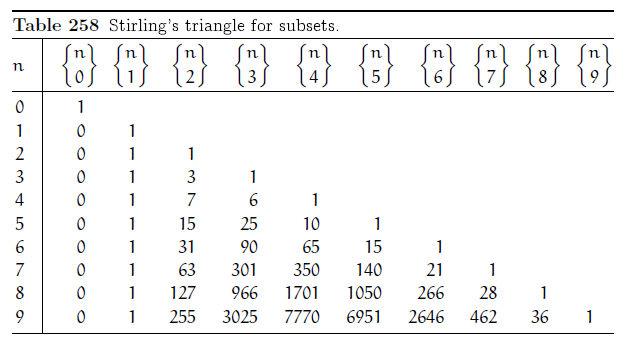
\includegraphics[scale=0.7]{images/stirling_2nd.png}
\caption{Page1}
\end{figure}

An ordinary power can then be expressed in terms of falling factorials
as follows

\begin{equation}
x^n = \sum_k {n \brace k} x^{\underline{n}}
\end{equation}
